For this experiment we will not include the TSNE plots.
\begin{figure}[!ht]
  \centering
  % 0.518 and 0.539
  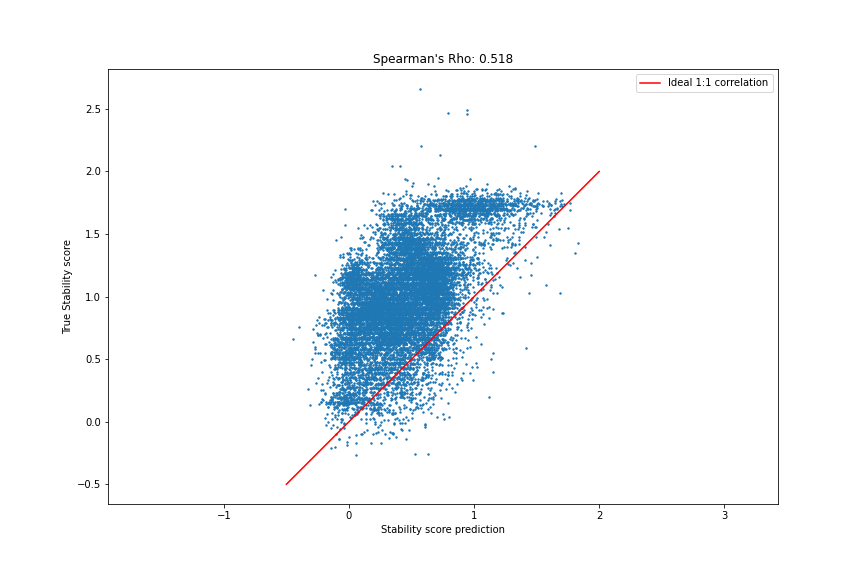
\includegraphics[width=0.49\linewidth]{latex/imgs/spearman_2_layer_05_drop_final.png}
  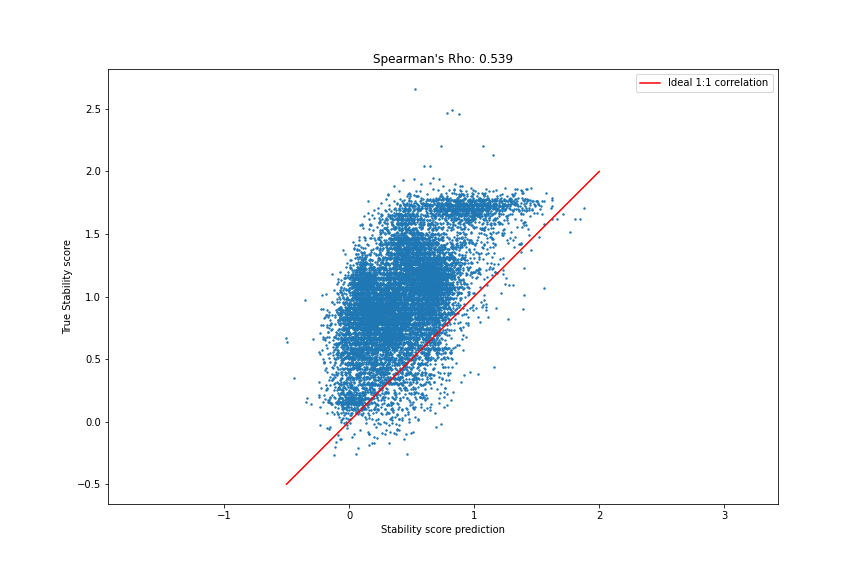
\includegraphics[width=0.49\linewidth]{latex/imgs/spearman_2_layer_05_drop_minloss.png}
  % 0.400 and 0.427
  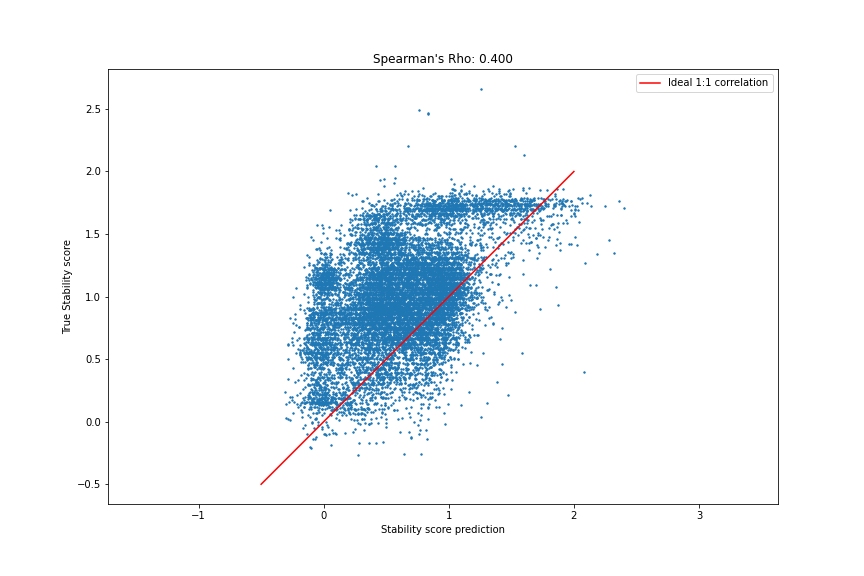
\includegraphics[width=0.49\linewidth]{latex/imgs/spearman_2_layer_no_drop_final.png}
  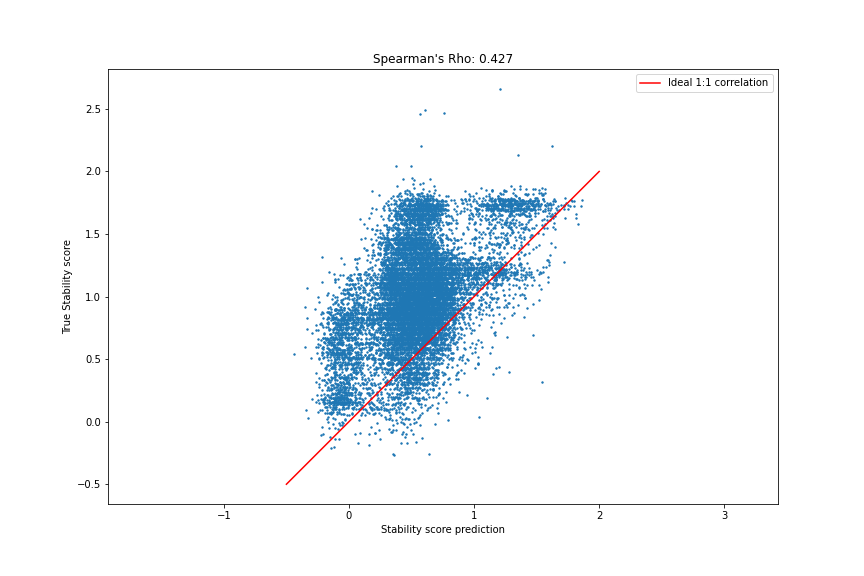
\includegraphics[width=0.49\linewidth]{latex/imgs/spearman_2_layer_no_drop_minloss.png}
  % 0.605 and 0.592
  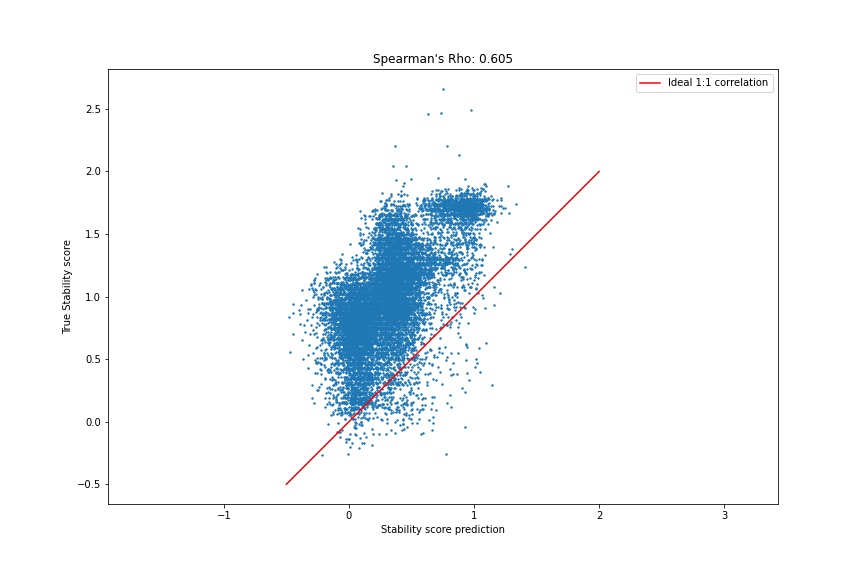
\includegraphics[width=0.49\linewidth]{latex/imgs/spearman_1_layer_no_schedule_512_final.png}
  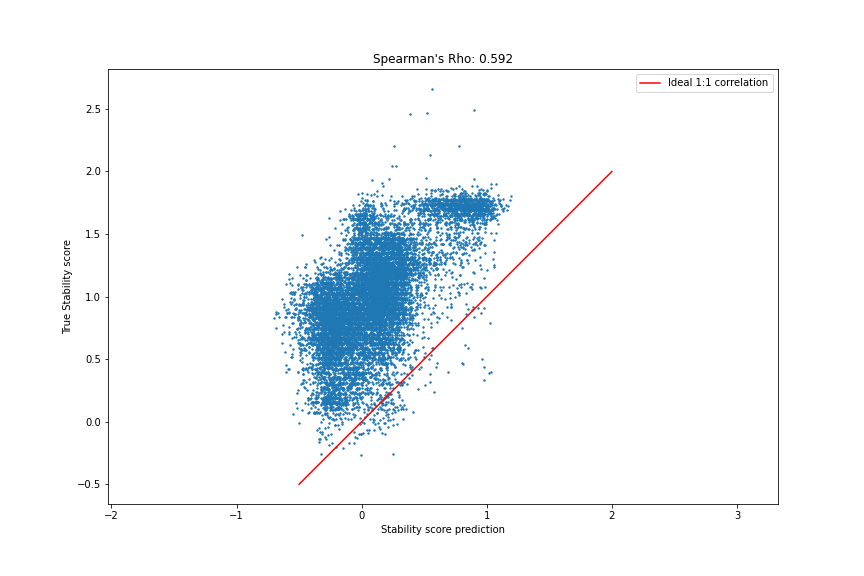
\includegraphics[width=0.49\linewidth]{latex/imgs/spearman_1_layer_no_schedule_512_minloss.png}
  % 0.428 and 0.414
  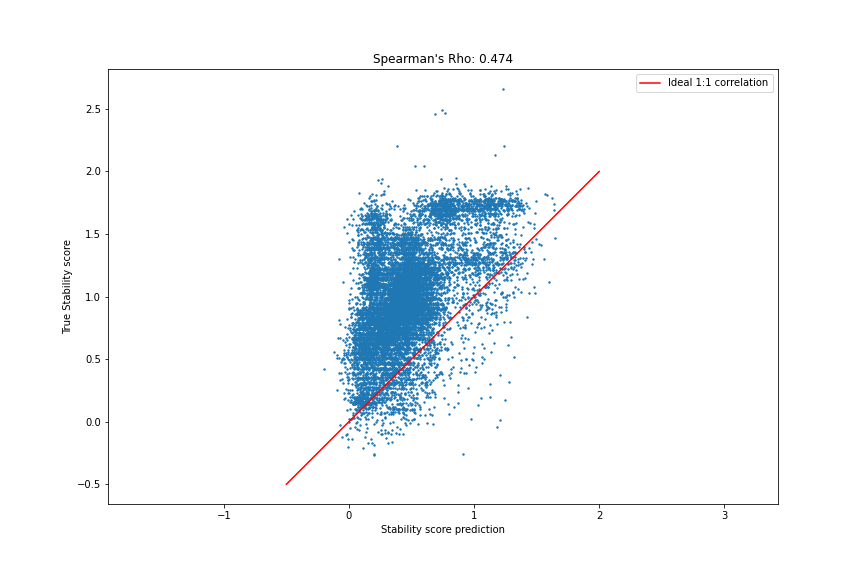
\includegraphics[width=0.49\linewidth]{latex/imgs/spearman_1_layer_with_schedule_512_final.png}
  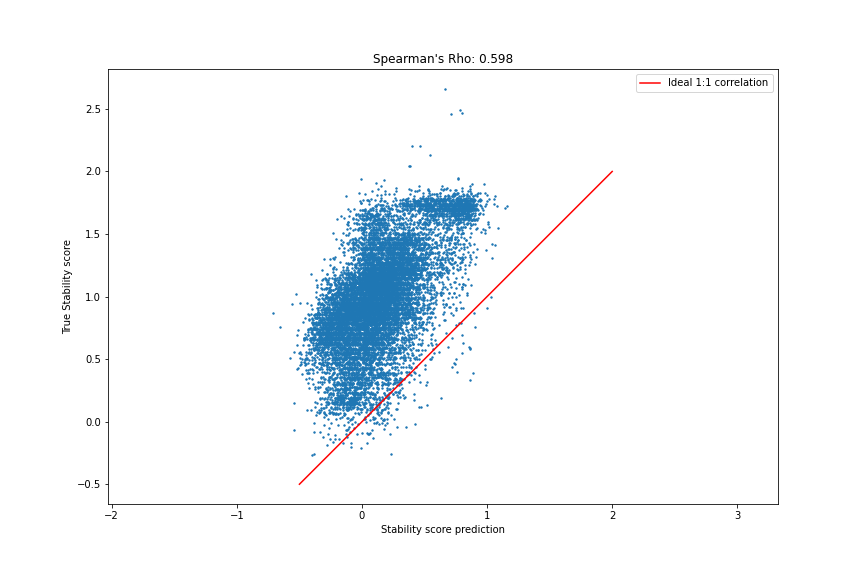
\includegraphics[width=0.49\linewidth]{latex/imgs/spearman_1_layer_with_schedule_512_minloss.png}
  % 0.435 and 0.424
  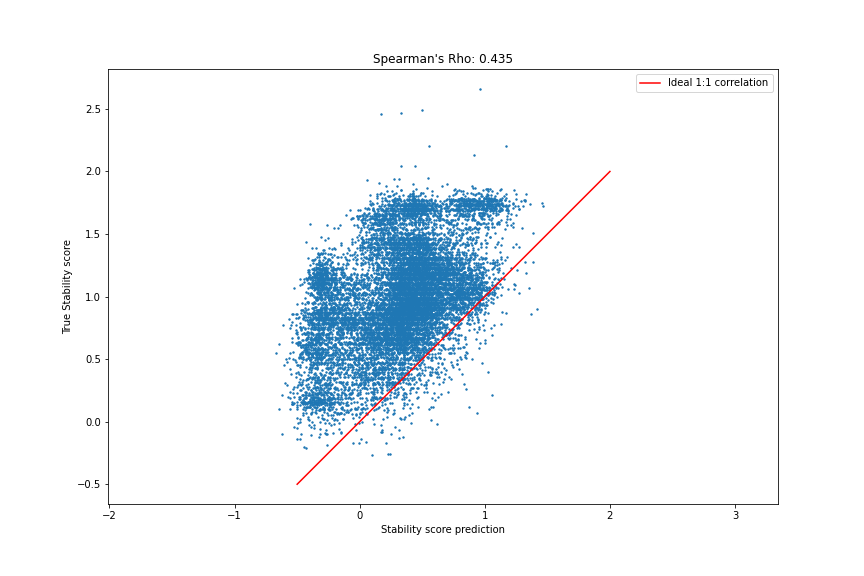
\includegraphics[width=0.49\linewidth]{latex/imgs/spearman_1_layer_with_schedule_256_final.png}
  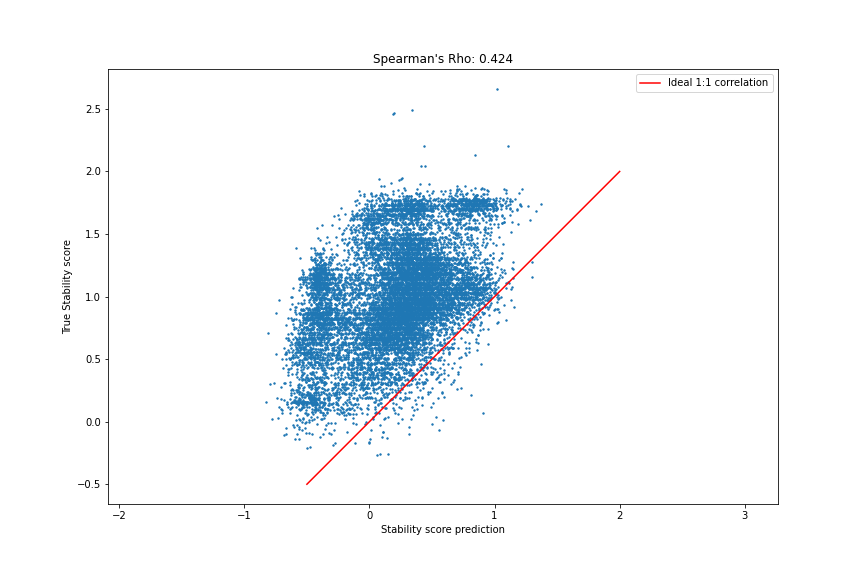
\includegraphics[width=0.49\linewidth]{latex/imgs/spearman_1_layer_with_schedule_256_minloss.png}
  % 0.507 and 0.627
  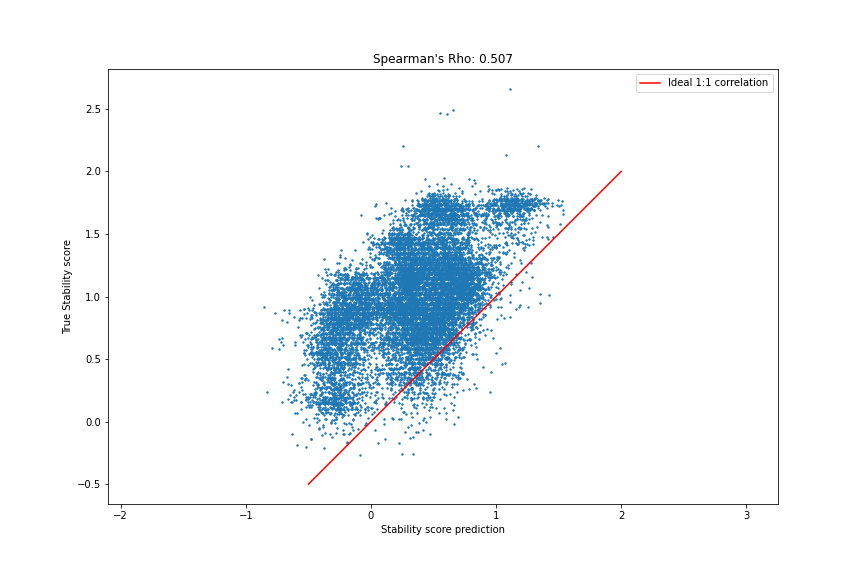
\includegraphics[width=0.49\linewidth]{latex/imgs/spearman_1_layer_with_schedule_1024_final.png}
  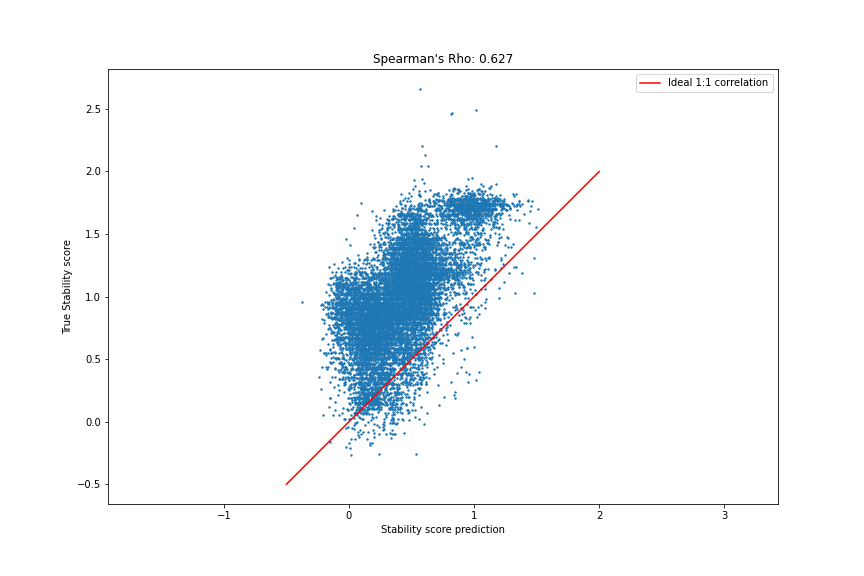
\includegraphics[width=0.49\linewidth]{latex/imgs/spearman_1_layer_with_schedule_1024_minloss.png}
  \caption{TSNE dimensionality reduction  and Spearman's rho data plots of the two models. Left is without no learning rate schedule, right is with the schedule mention in the experiments section.}
\end{figure}

\begin{table}[!ht]
\begin{tabular}{|l|lll|}
\hline
                                      &                                                     & Final Models                       &                \\ \cline{2-4} 
                                      & \multicolumn{1}{l|}{Next token prediction accuracy} & \multicolumn{1}{l|}{Test Loss}     & Spearman's rho \\ \hline
2-layer, 50\% dropout, 512 features   & \multicolumn{1}{l|}{13.02\%}                        & \multicolumn{1}{l|}{2.82}          & 0.518          \\ \hline
2-layer, no dropout, 512 features     & \multicolumn{1}{l|}{13.03\%}                        & \multicolumn{1}{l|}{2.83}          & 0.400          \\ \hline
1-layer, no lr schedule, 512 features & \multicolumn{1}{l|}{13.34\%}                        & \multicolumn{1}{l|}{2.83}          & \textbf{0.605} \\ \hline
1-layer, 256 features                 & \multicolumn{1}{l|}{11.41\%}                        & \multicolumn{1}{l|}{2.86}          & 0.435          \\ \hline
1-layer, 512 features                 & \multicolumn{1}{l|}{12.43\%}                        & \multicolumn{1}{l|}{2.84}          & 0.428          \\ \hline
1-layer, 1024 features                & \multicolumn{1}{l|}{\textbf{14.37\%}}               & \multicolumn{1}{l|}{\textbf{2.79}} & 0.507          \\ \hline
\end{tabular}
\end{table}
\begin{table}[!ht]
\begin{tabular}{|l|lll|}
\hline
                                      &                                                     & Minloss models                     &                \\ \cline{2-4} 
                                      & \multicolumn{1}{l|}{Next token prediction accuracy} & \multicolumn{1}{l|}{Test Loss}     & Spearman's rho \\ \hline
2-layer, 50\% dropout, 512 features   & \multicolumn{1}{l|}{13.03\%}                        & \multicolumn{1}{l|}{2.82}          & 0.539          \\ \hline
2-layer, no dropout, 512 features     & \multicolumn{1}{l|}{13.78\%}                        & \multicolumn{1}{l|}{2.81}          & 0.427          \\ \hline
1-layer, no lr schedule, 512 features & \multicolumn{1}{l|}{13.36\%}                        & \multicolumn{1}{l|}{2.83}          & 0.592          \\ \hline
1-layer, 256 features                 & \multicolumn{1}{l|}{11.40\%}                        & \multicolumn{1}{l|}{2.87}          & 0.424          \\ \hline
1-layer, 512 features                 & \multicolumn{1}{l|}{12.43\%}                        & \multicolumn{1}{l|}{2.85}          & 0.414          \\ \hline
1-layer, 1024 features                & \multicolumn{1}{l|}{\textbf{14.22\%}}               & \multicolumn{1}{l|}{\textbf{2.80}} & \textbf{0.627} \\ \hline
\end{tabular}
\end{table}